
\section{Intersections, intention and scenarios}
\label{sec:intro_intersections}
When it comes to the scenarios considered in this work. This section aims to clarify the use of the words' intersection, intention and scenario.
% When a pedestrian approach a crossing they have been taught at a young age to look at both sides of the road before crossing. The same apply for a human driver approaching an intersection. 
% When a human driver approach an intersection, it is natural to observe the environment to identify the traffic light, signs and other approaching vehicles. Then assess the situation, who has the right of way? 

% The intention of the other driver can be guided by the 
% Recently nontraditional intersections are also becoming increasingly popular. The goal of these designs is to reduce the number and/or severity of conflict points by altering the customary vehicular paths at the intersection. In light of the increased focus on and occurrence of these intersection types, it is expected that the application of nontraditional designs will continue to spread.

\begin{figure}[h]
	\centering
	\begin{subfigure}[t]{0.48\columnwidth}
		\centering
		\begin{tikzpicture}
			% Crossing
			\def\crossleftx{-2}
			\def\crossrightx{2}
			\def\crosstopy{2}
			\def\crossboty{-2}
			\def\roadwidth{0.5}

			\draw (0,0) circle (2pt);
			\node at (1.2, 0.2) {conflict point};
			\draw[thick] (\crossleftx, \roadwidth) -- (-\roadwidth, \roadwidth) -- (-\roadwidth, \crosstopy);
			\draw[thick] (\crossleftx, -\roadwidth) -- (-\roadwidth, -\roadwidth) -- (-\roadwidth-\roadwidth, \crossboty);
			\draw[thick] (\roadwidth, \crosstopy) -- (\roadwidth, \roadwidth) -- (\crossrightx, \roadwidth);
			\draw[thick] (\roadwidth-\roadwidth, \crossboty) -- (\roadwidth, -\roadwidth) -- (\crossrightx, -\roadwidth);

			% 	cars
			\node[inner sep=0pt] (ego_car) at (\crossleftx+0.5,0)
			{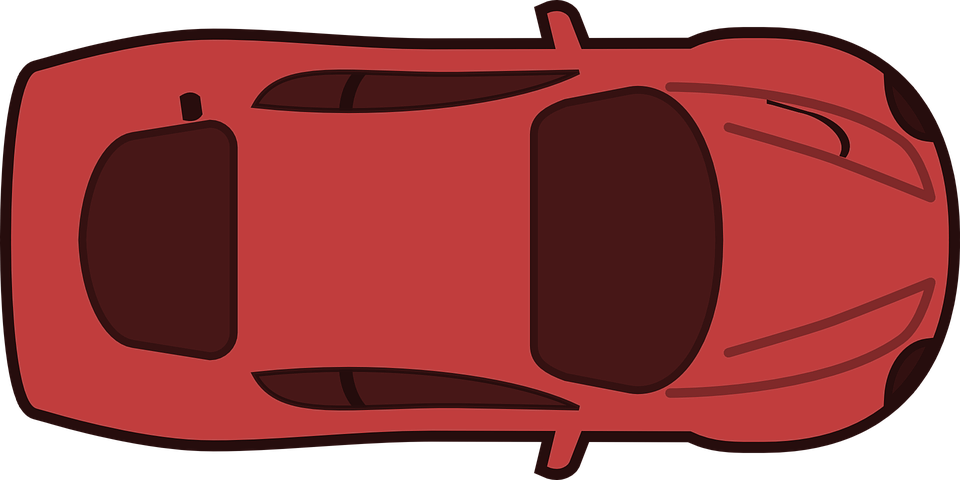
\includegraphics[width=.18\textwidth, angle=0]{figures/ego_car_top_down.png}};

			\node[inner sep=0pt] (target_car) at (0,\crosstopy-0.5)
			{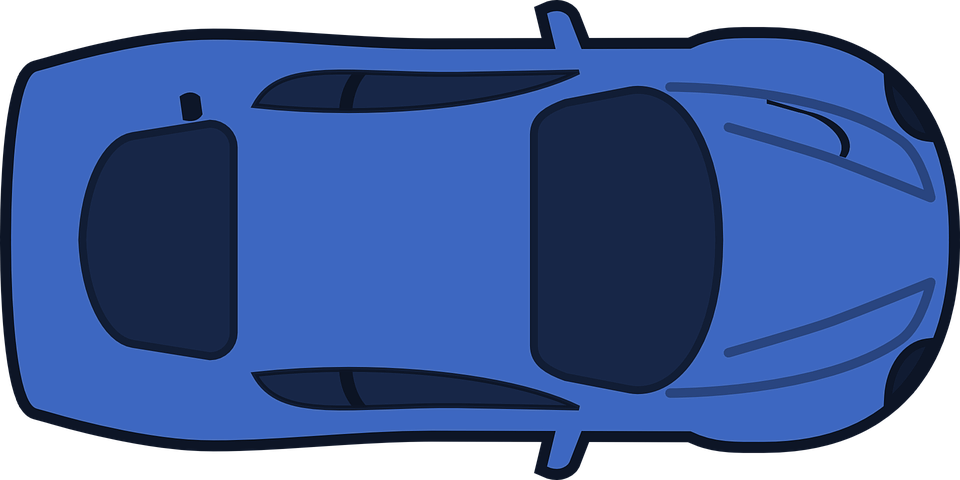
\includegraphics[width=.18\textwidth, angle=-90]{figures/target_car_top_down.png}};

			\node[inner sep=0pt] (target_car) at (-.1,-0.8)
			{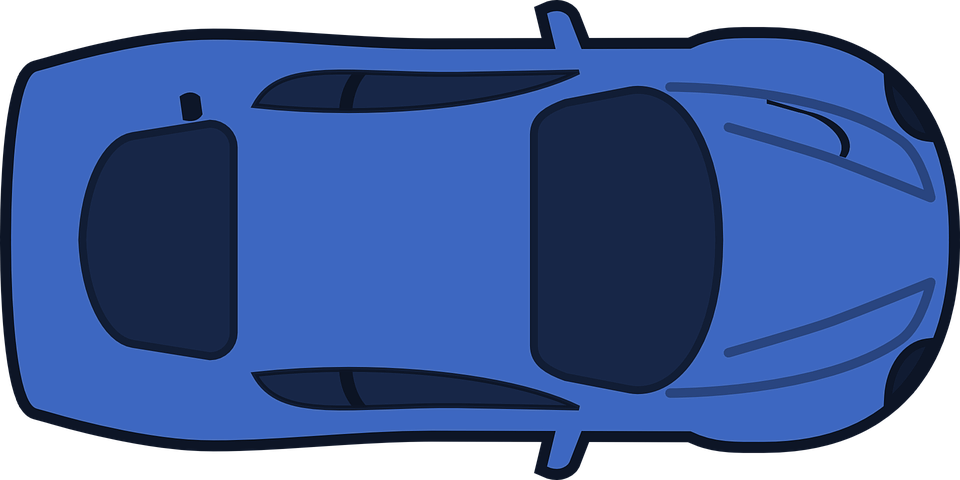
\includegraphics[width=.18\textwidth, angle=-110]{figures/target_car_top_down.png}};


		\end{tikzpicture}
		\caption{Single intersection}
\end{subfigure}%
	~ 
	\begin{subfigure}[t]{0.48\columnwidth}
		\centering
		\begin{tikzpicture}
			% Crossing
			\def\crossleftx{-2.5}
			\def\crossrightx{2.5}
			\def\crosstopy{2}
			\def\crossboty{-2}
			\def\roadwidth{0.5}

			\draw (-0.5,0) circle (2pt);
			\draw (0.5,0) circle (2pt);
			% \node at (0.7, 0.2) {crossing point$^1$};
			\draw[thick] (\crossleftx, \roadwidth) -- (-\roadwidth-0.5, \roadwidth) -- (-\roadwidth-0.5, \crosstopy);
			\draw[thick] (\crossleftx, -\roadwidth) -- (-\roadwidth-0.5, -\roadwidth) -- (-\roadwidth-0.5, \crossboty);
			\draw[thick] (0, \crosstopy) -- (0, \roadwidth);
			\draw[thick] (0, -\roadwidth) -- (0, \crossboty);
			\draw[thick] (\roadwidth+0.5, \crosstopy) -- (\roadwidth+0.5, \roadwidth) -- (\crossrightx, \roadwidth);
			\draw[thick] (\roadwidth+0.5, \crossboty) -- (\roadwidth+0.5, -\roadwidth) -- (\crossrightx, -\roadwidth);

			% 	cars
			\node[inner sep=0pt] (ego_car) at (\crossleftx+0.5,0)
			{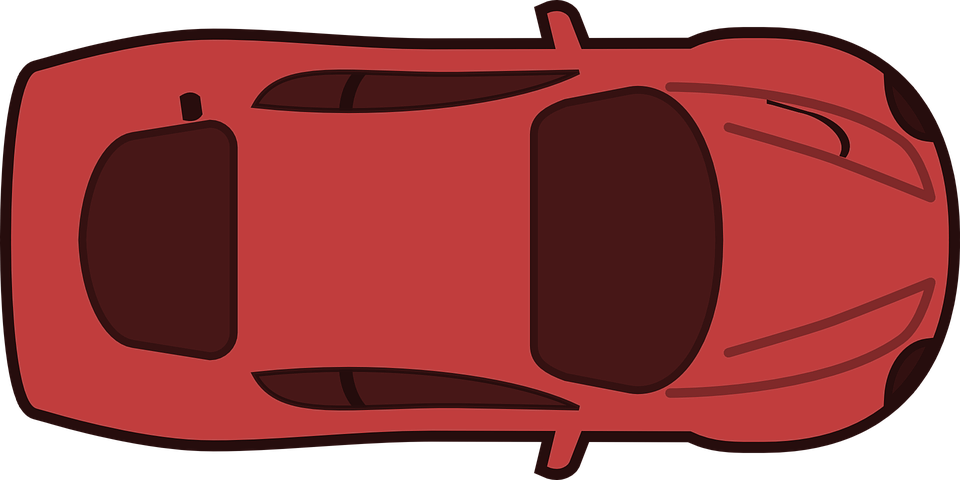
\includegraphics[width=.18\textwidth, angle=0]{figures/ego_car_top_down.png}};

			\node[inner sep=0pt] (target_car) at (-0.5,\crosstopy-0.5) {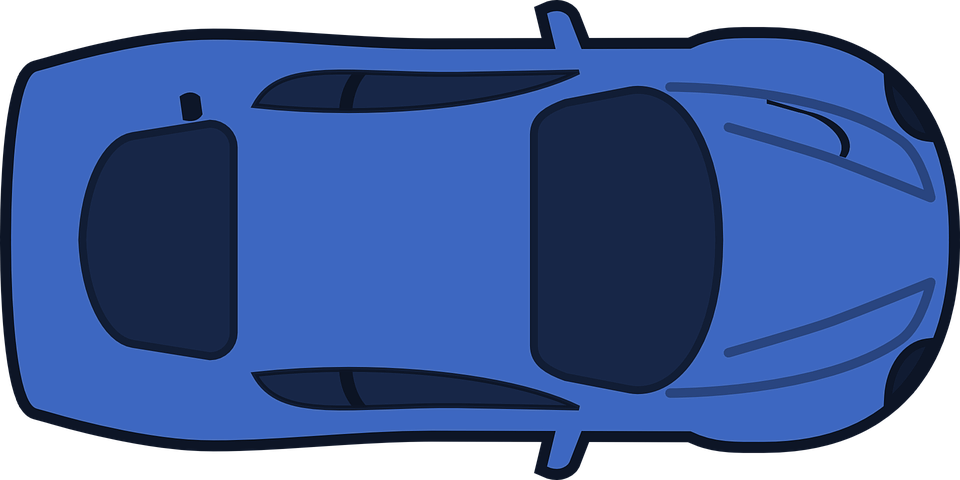
\includegraphics[width=.18\textwidth, angle=-90]{figures/target_car_top_down.png}};

			\node[inner sep=0pt] (target_car_2) at (0.5,\crossboty+0.5) {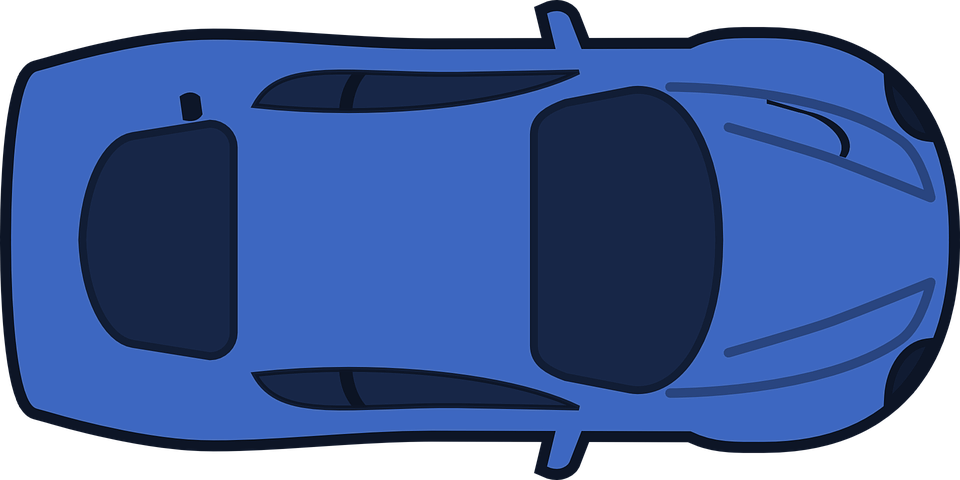
\includegraphics[width=.18\textwidth, angle=90]{figures/target_car_top_down.png}};

		\end{tikzpicture}
		\caption{Double intersection}
	\end{subfigure}

	\caption{Examples of different intersections}
	\label{fig:example_intersections}
\end{figure}
Let's begin by defining the terms 'intersection,' 'intention,' and 'scenario' within the context of this study.
An intersection refers to the geometric layout of roads intersecting each other, encompassing elements such as the number of junctions, conflict points, turns, and angles of incidence, as illustrated in Figure~\ref{fig:example_intersections}. 
Intersections can be categorized as signalized or unsignalized. A signalized intersection is equipped with mechanisms to designate the right-of-way, such as regulatory signs (e.g., STOP or YIELD) or traffic signals, while an unsignalized intersection lacks such features. However, as emphasized in the introduction, human drivers do not always adhere strictly to these right-of-way rules, which can result in accidents. Therefore, this thesis defines intentions as the anticipated actions of other vehicles in the future, such as stopping, cautiously slowing down, or proceeding through the intersection.

\begin{figure}[h]
	% \mbox{\parbox{\textwidth}{
	% \centering
	% % \vspace{0.3cm}
	% 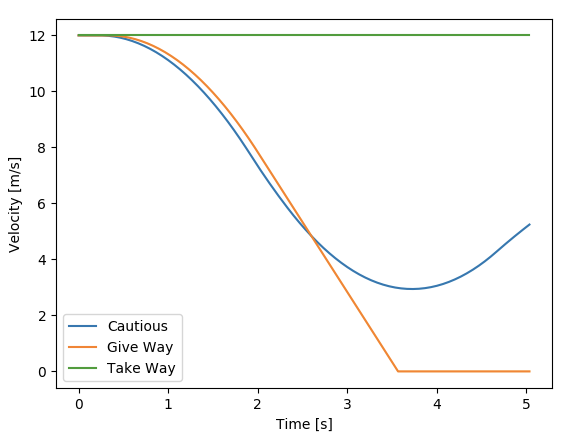
\includegraphics[width=0.6\columnwidth]{YourThesis/papers/mpc/figures/velocity_profiles_agents.png}
	% }}
	\centering
	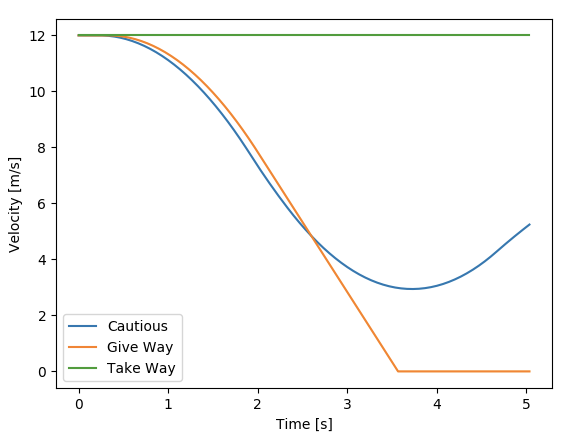
\includegraphics[width=0.6\columnwidth]{YourThesis/papers/mpc/figures/velocity_profiles_agents.png}

	\caption{An illustration showing velocity profiles for agents with three distinct intentions. Each agent shares the same initial position and velocity while approaching a common intersection.}
	\label{fig:intro_intention_profiles}
	% \vspace{-0.3cm}
\end{figure}

Figure \ref{fig:intro_intention_profiles} illustrates how velocity profiles can differ for three different intentions. In this example, distinguishing between the 'give way' and 'take way' intentions is straightforward, as the velocity begins to decelerate at time $0$. However, identifying the 'cautious' intention poses a challenge, as the agent cannot be certain until the other vehicle comes to a complete stop.

If intentions are known, intersections can be treated as unsignalized, as the right-of-way can be inferred from the intentions rather than relying solely on infrastructure. This approach ensures safety even in situations where another vehicle disregards traffic rules, such as running a red light, as a cautious agent will prioritize safety and stop accordingly.

\section{The intersection problem}
\begin{figure}
	\mbox{\parbox{\textwidth}{
		\centering
		\begin{tikzpicture}
			\def\xstart{-7};

			\coordinate (p) at (3,0);
			\foreach \n/\w/\c in {z0/2/green,z1/2/red,z2/2.5/orange,z3/3.5/blue}{
				\node[rectangle,
				draw=none,
				anchor=east,
				text = black,
				fill = \c!60,
				minimum width = \w cm, 
				minimum height = 2cm] 
				(n) at (p) {\Huge \n};
				
				\coordinate (p) at (n.west);
			}

			% Crossing
			\draw[line width=0.5mm] (\xstart, 1) -- (-1, 1) -- (-1, 5);
			\draw[line width=0.5mm] (\xstart, -1) -- (-1, -1) -- (-1, -2);
			\draw[line width=0.5mm] (1, 5) -- (1, 1) -- (3, 1);
			\draw[line width=0.5mm] (1, -2) -- (1, -1) -- (3, -1);
			
			% cars
			\node[inner sep=0pt] (ego_car) at (-7,0)
			{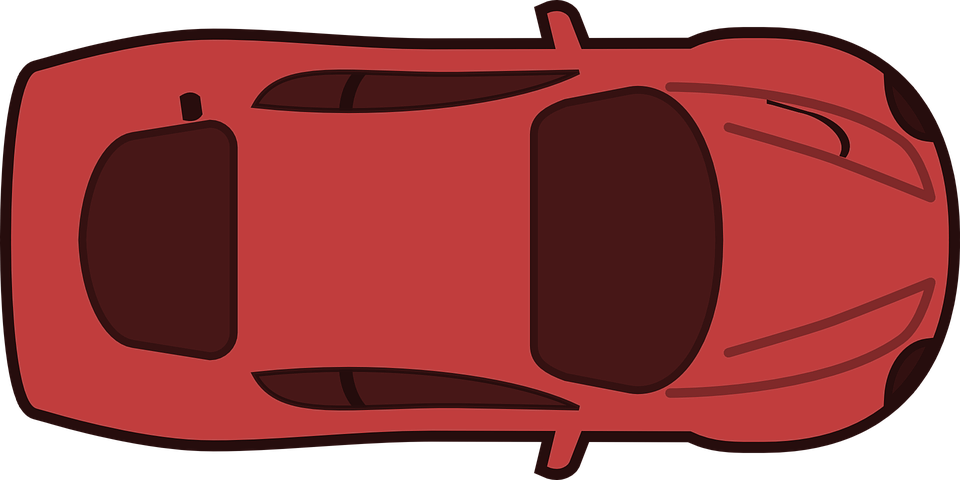
\includegraphics[width=.18\textwidth, angle=0]{figures/ego_car_top_down.png}};
			\node[inner sep=0pt] (target_car) at (0,4)
			{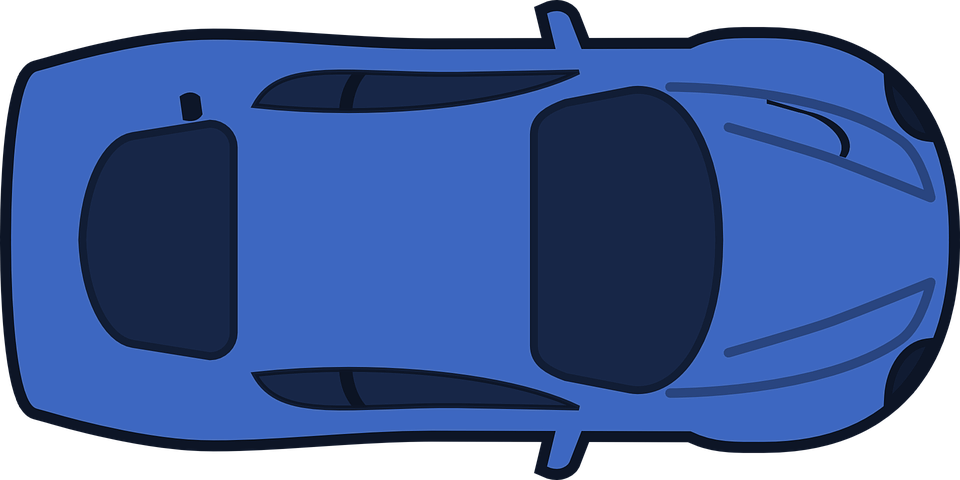
\includegraphics[width=.18\textwidth, angle=-90]{figures/target_car_top_down.png}};

	\end{tikzpicture}
	}}
	\caption{Intersection scenario divided into zones describing what is required of the decision maker in different zones}
	\label{fig:zones}
\end{figure}

With the \gls{mdp} defined, the path of the ego vehicle can be segmented into four zones as shown in Figure~\ref{fig:zones}. Starting from the end, Zone 0 represents the 'safe zone,' where the ego vehicle is out of danger and can resume nominal driving. Zone 1 is the 'conflict zone,' where a collision with another vehicle is possible. Zone 2, the 'critical decision zone,' is the final opportunity for the vehicle to either stop or proceed through the intersection. The size of zone 2 is determined by the minimum distance required for the vehicle to come to a complete stop before entering the conflict zone, ensuring sufficient time for safe decision-making. Lastly, Zone 3, the 'information gathering zone,' is situated furthest from the intersection. Here, the agent can observe how other vehicles behave over time to estimate their intentions.

The goal is to reach Zone 0. To achieve this, the agent aims to minimize the time spent in Zone 1 if there is a chance of intersection with another car. Our actions are formulated as short-term goals, designed for comfortable use with lower acceleration rates. The size of Zone 2 depends on the vehicle's current speed, which is influenced by its behavior in Zone 3.

Now, two conflicting strategies emerge: to minimize time in Zone 1, the agent desires a high speed entering the intersection. However, it also seeks a low speed to reduce the size of Zone 2 and the critical decision period. If the intentions of other vehicles are known, the stochasticity in Zone 1 would be eliminated, transforming the problem into a scheduling task aimed at creating a velocity profile that minimizes the time required to cross. However, since the intentions of other vehicles are stochastic, reinforcement learning offers a promising approach to address this uncertainty and optimize decision-making in dynamic traffic scenarios.
